\documentclass{article}
\usepackage[margin=1in]{geometry}
\usepackage{amsmath,amsthm,amssymb}
\usepackage{bbm,enumerate,mathtools}
\usepackage{tikz,pgfplots}
\usepackage{chessboard}
\usepackage[hidelinks]{hyperref}
\usepackage{multicol} % Problem 35
\usepackage{xstring} % Difficulty command
\usetikzlibrary{shapes.geometric}

\newenvironment{question}{\begin{trivlist}\item[\textbf{Question.}]}{\end{trivlist}}
\newenvironment{note}{\begin{trivlist}\item[\textbf{Note.}]}{\end{trivlist}}
\newenvironment{references}{\begin{trivlist}\item[\textbf{References.}]}{\end{trivlist}}
\newenvironment{related}{\begin{trivlist}\item[\textbf{Related.}]\end{trivlist}\begin{enumerate}}{\end{enumerate}}

\newcommand\score[1]{
\pgfmathsetmacro\pgfxa{#1+1}
\tikzstyle{scorestars}=[
  star,
  star points=5,
  star point ratio=2.25,
  draw,
  inner sep=3pt,
  anchor=outer point 5
]
  \begin{tikzpicture}[baseline]
    \draw[opacity=0] (0,-0.5) rectangle (0,0.2); % Workaround for whitespace at the bottom.
    \foreach \i in {1,...,4} {
      \pgfmathparse{(\i<=#1?"yellow":"gray")}
      \edef\starcolor{\pgfmathresult}
      \draw (\i*4.5ex,0) node[name=star\i,scorestars,fill=\starcolor]  {};
    }
  \end{tikzpicture}
}

\newcommand{\difficulty}[1]{%
  \IfEqCase{#1}{%
      {1}{
        
\begin{tikzpicture}[scale=0.7, baseline=0.9mm]%
          \definecolor{slopegreen}{rgb}{0.0, 0.5, 0.0}%
          \fill[slopegreen] (0.5,0.5) circle (0.5);%
        \end{tikzpicture}%
      }%
      {2}{
        
\begin{tikzpicture}[scale=0.7, baseline=0.9mm]%
          \definecolor{slopeblue}{rgb}{0.0, 0.44, 1.00}
          \fill[slopeblue] (0,0) rectangle (1,1);%
        \end{tikzpicture}%
      }%
      {3}{
\begin{tikzpicture}[scale=0.7, baseline=0.9mm]\fill (0,0.5)--(0.5, 0)--(1,0.5)--(0.5,1)--cycle; \end{tikzpicture}}%
      {4}{
\begin{tikzpicture}[scale=0.7, baseline=0.9mm]\fill (0.25,0)--(0,0.5)--(0.25,1)--(0.5,0.5)--cycle; \fill (0.75,0)--(0.5,0.5)--(0.75,1)--(1,0.5)--cycle;\end{tikzpicture}}%
      % you can add more cases here as desired
  }[\PackageError{difficulty}{Undefined difficulty level: #1}{}]%
}%
\newcommand{\rating}[2]{\difficulty{#1}\\\score{#2}\\}


\begin{document}
\rating{2}{2}
Starting with a row of $n$ coins all heads up, repeatedly flip over a coin which
is heads and its neighbor to the right. If the chosen coin is the rightmost
coin, there is no neighbor to flip.

\begin{figure}[ht!]
  \centering
  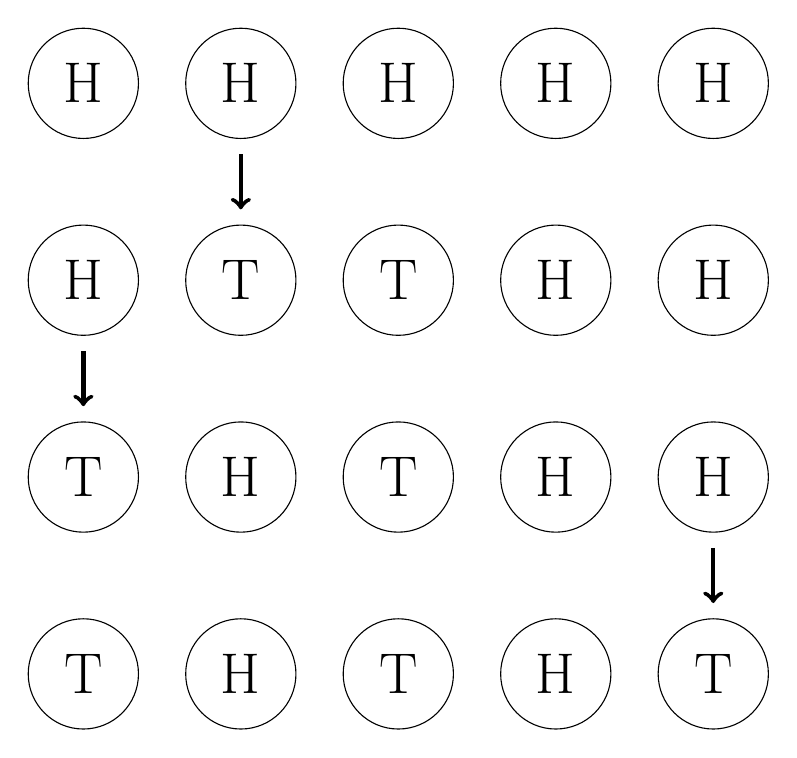
\begin{tikzpicture}
    \foreach \i/\f in {0/H,1/H,2/H,3/H,4/H} {
      \draw (2*\i, 0) circle (0.7) node {\huge\f};
    }
    \draw[ultra thick, ->] (2, -0.9)--(2, -1.6);
    \foreach \i/\f in {0/H,1/T,2/T,3/H,4/H} {
      \draw (2*\i, -2.5) circle (0.7) node {\huge\f};
    }
    \draw[ultra thick, ->] (0, -3.4)--(0, -4.1);
    \foreach \i/\f in {0/T,1/H,2/T,3/H,4/H} {
      \draw (2*\i, -5) circle (0.7) node {\huge\f};
    }
    \draw[ultra thick, ->] (8, -5.9)--(8, -6.6);
    \foreach \i/\f in {0/T,1/H,2/T,3/H,4/T} {
      \draw (2*\i, -7.5) circle (0.7) node {\huge\f};
    }
  \end{tikzpicture}
  \caption{
    Since the sequence of coin flips strictly increases lexicographically
    (with $T > H$), the process must eventually halt.
  }
\end{figure}
\begin{question}
  If the puzzle is modified so that when a coin is chosen, either the right or
  left neighbor is chosen (with probability $p$ and $1 - p$ respectively),
  what is the optimum strategy for maximizing the total number of flips?
\end{question}

\begin{related}
  \item What is the strategy for minimizing the number of flips?
  \item What is the expected number of total flips under optimal play?
  \item What if the direction is randomly chosen, and then you choose which
  coin to flip? (i.e. you know the direction before you make your choice.)
  \item What if the (infinite) sequence of choices have to all be made ahead of
  time?
  \item What if this is done on a different geometry, such as a circle or grid?
  \item What if one, neither, or both neighbors have some probability of being
    flipped?
  \item What if coins have more than two states? (e.g dice instead of coins)
  \item What if you can flip over a contiguous section of heads?
\end{related}

\begin{references}
  \item Problem 79.
\end{references}

\end{document}
